\documentclass[12pt]{article}

\usepackage[pdftex]{graphicx}
\usepackage{amsmath}
\usepackage[round]{natbib}

\usepackage{fullpage}

\usepackage{palatino}
\usepackage{mathpazo}
\usepackage{rotating}

\usepackage[mathlines]{lineno}
\usepackage{setspace}

\clubpenalty=10000
\widowpenalty=10000
\displaywidowpenalty=3000
\predisplaypenalty=3000
\postdisplaypenalty=2000

\begin{document}

\vfill
\noindent
{\large\bfseries Spreading and mixing in near-field river plumes}\\
\noindent
{\scshape Robert D. Hetland}\\
\noindent
{\footnotesize Dept. of Oceanography, Texas A\&M University, College Station, TX}

% \doublespacing
% \linenumbers

\begin{abstract}
  \small{Lorem ipsum dolor sit amet, consectetur adipisicing elit, sed do eiusmod tempor incididunt ut labore et dolore magna aliqua. Ut enim ad minim veniam, quis nostrud exercitation ullamco laboris nisi ut aliquip ex ea commodo consequat. Duis aute irure dolor in reprehenderit in voluptate velit esse cillum dolore eu fugiat nulla pariatur. Excepteur sint occaecat cupidatat non proident, sunt in culpa qui officia deserunt mollit anim id est laborum.}
\end{abstract}


\section{Introduction}

The estuary/river plume system is a mixing region where terrestrial fresh water is transformed into to brackish ocean seawater. While in some large systems, this brackish seawater may be observed thousands of kilometers from the source, generally the strong gradients in salinity are concentrated either within the estuary or near-field river plume. The near-field plume is often associated with energetic flows -- Froude numbers above one -- and intense mixing, but more generally can be considered to be the region of rapid transition in the character of the estuarine outflow. Though both both estuaries and near-field plumes can be characterized by large gradients in salinity over an area small compared to the continental shelf, and terrestrial water passing to the ocean must pass through both regions, estuaries and river plumes are often treated separately. One reason may be geographic; estuaries have clear boundaries, distinct ecosystems, and may be next to population centers that care about local water quality. Near-field river plumes on the other hand are ephemeral, have no distinct boundaries, and are not associated with any particular distinct ecosystem. Near-field plumes also have distinct dynamics -- supercritical flow detached from the bottom and not constrained latterally by the coastline -- with small timescales -- usually a few hours.

% Motivation/challenges
% \begin{itemize}
%   \item Rapid transition/dilution
%   \item Strong gradients
%   \item Small scale (challenges for parameterization vs. resolution)
%   \item High Froude number flows
%   \item Possible very small scale, O(1) aspect flows near the front of unknown importance
% \end{itemize}


% \paragraph{Estistance 
Not every river or estuary entering into the coastal ocean has an associated near-field plume. The mouth of the estuary needs to be narrow enough for hydraulic control to affect the outflow. For wide estuary mouths, rotation will become an important factor in determining the structure of the outflow. If the estuarine flow is given sufficient space, the bouyant estuarine outflow will form a trapped boundary current, hugging the righthand coast as the flow travels seaward. This process breaks the hydraulic control, as the structure of the flow exiting the estuary is determined by rotating dynamics, and not hydraulics. Thus, the first criterion for a near-field plume to exist is that the mouth be narrow compared to the deformation radius, or that the Kelvin number, $K$ -- the ratio between the width of the estuary mouth, $W$ and the deformation radius, $R_d = \sqrt{g' H} f^{-1}$ -- be small, $K = W R_d^{-1} \ll 1$. (Garvine, HDHM)

Another condition for the existence of a substantial near-field plume is the presence of relatively quiescent receiving waters. This can be quantified by comparing the potential energy anomaly provided by the buoyant outflow to the dissipative energy associated with winds and tides \citep{pritchard.huntley:02}; storms and strong tides can mix away a plume before it forms or strongly impact its evolution. In practice, because river discharge varies over many orders of magnitude across different systems and seasons, it is the input of potential energy by the buoyant outflow that is the strongest determining factor in forming a robust plume; large river systems generally have well defined plumes.

The near-field plume is part of a series of regions that process fresh water from rivers by mixing and transporting water through the estuary/river plume system. The near-field plume is an important region because, though small relative to the other regions of the estuary/plume system, mixing can be intense, and a significant fraction of the total mixing that river water experiences through the estuary/plume system can occur in the near-field plume. In the next section, the dynamical regions surrounding the near-field river plume are examined in more detail.

\section{Dynamical elements}

Estuarine outflow defines the initial salinity and volume transport of the coastal plume.  If the mouth is narrow, a near-field plume will form, and salinity and momentum will be rapidly modified by intense mixing. Otherwise, the estuarine outflow will form a buoyancy driven coastal current where properties will change much more slowly; this type of flow is more a continuation of the flow patterns in the estuary, and is not as dynamically distinct as a near-field plume. A key difference between these two features is that the near-field plume is supercritical, with $Fr = U \sqrt{g' h} > 1$, so that momentum in the near-field plume is strong. The strong momentum in the near-field plume inhibits the immidiate formation of a rotating coastal current, and often directs the flow offshore. 

As the near-field plume collapses and transitions back to subcritical flow, rotation becomes a dominant factor, and the flow is redirected toward the coast. This creates a recirculating bulge that has been the focus of a number of laboratory \citep{avicola.huq:03b,horner-devine.ea:06}, numerical \citep{fong.geyer:02,isobe:05}, and observational \citep{horner-devine:09,kudela.ea:10} studies. Connections between the near-field plume and the recirculating bulge are not yet clear, but there are two potential interactions that can influence the near-field plume circulation. First, the transition from (non-rotating) near-field jet to (rotating) bulge region is not abrupt, and rotational effects are important at the end of the near-field region \citep{cole.dissertation}; this may cause a shutdown in near-field plume spreading that then inhibits mixing. The second potential interaction is that the returning, up-coast flow in the recirculating bulge may interact with the near-field plume; the recirculating bulge water may place additional forces on the near-field plume, or modify the water that is entrained.

Downcoast of the bulge region, an along-shore coastal current forms \citep{} that may be affected by tides \citep{deboer.ea:08,pritchard.huntley:06} or winds \citep{fong.geyer:01,hetland:05,lentz:04,jurisa.chant:13}. Though this region is typically much larger than the near-field plume, the influence of the near-field is important because the estuarine outflow may be significantly modified in the near-field. Many theoretical studies relate the structure of the coastal current flow to properties of the estuarine outflow, but in practice this should be related instead to the water properies leaving the near-field plume.

% \paragraph{Liftoff}
The initiation of the near-field plume is located at a point of internal hydraulic control. In practice this is usually bottom, topographic control from a tidal bar at the mouth of an estuary, like in the Merrimack \citep{macdonald.ea:07} or Fraser \citep{macdonald.geyer:05} rivers, however there are also cases where the control is created at the end of the jetties, where the channel width goes from finite to infinite, as in the case of some of the Mississippi Delta passes \citep{wright.coleman:71}. After the hydraulic control point, the seaward flow transitions to supercricital, and this supercritical flow characterizes the near-field plume.

Supercritical flow influences the near-field plume in two ways. First, high Froude numbers imply low bulk Richardson numbers, where $Ri_b = g' h U^{-2} = Fr^{-2}$ which in turn means the flow could be susceptible to internal Kelvin-Hemholtz instabilities. Second, the supercritical flow is often associated with flow separation at the estuary mouth. This can be influenced by the geometry of the estuary mouth; for example, jetties will tend to favor flow separation more than a gradually widening, funnel-shaped estuary mouth.


% \paragraph{spreading}

If a near-field plume separates from the coastline, the plume will be able to freely spread. The spreading rate will be twice the internal gravity wave speed, the edges of the plume will each expand in a direction away from the axis of the plume at a rate defined by the local internal phase speed \citep{hetland.macdonald:08}. Properties within the core of the plume are fairly constant in the lateral direction, and are primarily a function of the distance from the estuary mouth. As such, the spreading rate is also primarily a function of distance from the mouth, and does not significantly vary laterally across the plume. 

Note that if the plume does not separate, the geometry of the estuary and coastline will control the spreading rate instead of internal plume dynamics. In this case, a plume might look more like an expansion within an estuary, where the buoyant water maintains contact with the spreading boundaries \citep[see][]{,geyer.ea:17}; situations like this are also associated with elevated and intense mixing \citep{geyer.ea:10}.

% \paragraph{interior mixing}

Mixing in the near-field plume is driven by shear instabilities and can  e quite intense \citep{macdonald.ea:07}. In both the Merrimack and Columbia plumes, shear squared and stratification frequency squared can both exceed 0.1 s$^{-2}$, and turbulence dissipation rates well exceeding 10$^{-4}$~m$^{-2}$s$^{-3}$. A comparison between simulated and observed dissipation rates in the Merrimack river plume showed good agreement in magnitude and spatial distribution, most likely because the turbulence closure schemes work well under the strong signal of intense mixing. 

There is a process that may bias estimates of mixing in 0D mixing parameterizations, which includes essentially all modern turbulence closure schemes: there is some evidence that mixing may be enhanced even beyond what is expected from a local Richardson number-based parameterization through stretching and intensification of the vortex tubes. As Kelvin-Hemholz billows roll up, they are also stretched laterally by the spreading plume. This spreading can further enhance the lateral vorticity associated with the rolling billow, pumping more energy into the turbulent cascade \citep{macdonald.chen:12}. In practice, this effect may difficult to separate from variability in mixing within the plume, and a 0D mixing parameterization will reproduce the primary features terms of mixing strength and distribution. In other situations, for example when starts as vertical vorticity and is stretched laterally due to baroclinic shear, the intensification in the mixing can be a dominant process \citep[e.g.,][]{farmer.ea:02}.

\section{A simple near-field plume model}

Following \citep{hetland:10a}, the combined effects of a control point at the estuary mouth (i.e., liftoff), and subsequent plume spreading and mixing can be combined into a simple analytic model of the plume that can be used to approximate plume structure and estimate net mixing through the near-field plume. The key dependant variables are the density anomaly of the plume, $\Delta\rho$, the thickness of the active layer, $h$, the axial velocity, $u$, and the plume width, $W$; see Figure~\ref{fig:plume_vars}.

\begin{figure}
    \centering
    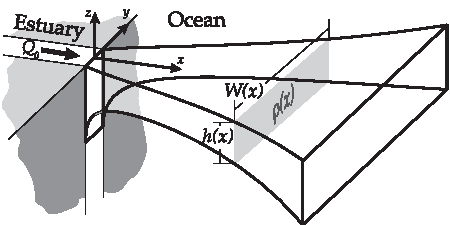
\includegraphics[width=5in]{Figures/plume_vars_flat.pdf}
    \caption{A schematic showing the variables in the simple model of a near-field plume.}
    \label{fig:plume_vars}
\end{figure}

Consider a rectangular estuary mouth, with width $W_0$. We will consider the estuarine outflow to be a single active layer over quiescent receiving waters, so will use a reduced gravity model. The outflow velocity is $u_0$, and the depth of the upper layer is $h_0$, both subject to the constraint that the flow is exactly critical \cite[i.e., the mouth acts as a constriction, see][]{armi.farmer:86, farmer.armi:86},
\begin{equation}
    \mathrm{Fr}\bigg|_{x=0} = \frac{u}{\sqrt{g' h}}\bigg|_{x=0} = 1 \quad ,
\end{equation}
where $g' = g \Delta \rho \rho_0$ is the reduced gravity, $g$ the gravitational acceleration, $\Delta \rho$ the buoyancy anomaly of the active layer, and  $\rho_0$ the density of the receiving waters.

As the plume evolves, it can entrain receiving waters into the active layer through an entrainment velocity, $w_e$. The entrainment velocity will be a parameterization of mixing processes, and could therefore be dependent on potential and kinetic energy anomalies in the flow; a more detailed discussion of the parameterization of entrainment follows, but for now it can be treated as an arbitrary function. The dynamical equation along the plume axis , $x$, following a slab of water exiting the estuary mouth, is
\begin{equation}
    \frac{Du}{Dt} = -(g' h)_x - \frac{w_e u}{h} \quad ,
\end{equation}
and conservation of density can be used to describe the evolution of the density anomaly following the slab of water
\begin{equation}
    \frac{D \Delta\rho}{Dt} = -\frac{w_e \Delta\rho}{h} \quad .
\end{equation}
The width of the slab will increase at twice the local gravity wave speed, as described above, requiring
\begin{equation}
    \frac{D W}{Dt} = 2 \sqrt{g' h}
\end{equation}
Finally, conservation of mass requires
\begin{equation}
    \frac{D}{Dt}\left( h u W \Delta\rho \right) = 0 \quad .
\end{equation}

Assuming that the plume is steady, the total derivative can be converted to an advection term
\begin{equation}
    \frac{D}{Dt} = u\frac{\partial}{\partial x} \quad .
\end{equation}
The equations can then be written as a set of ordinary differential equations
\begin{align}
\frac{\partial \Delta\rho}{\partial x} &= - \Delta \rho \frac{w_e}{u\,h} \label{eq:mass_sys}\\
\frac{\partial W}{\partial x} &=  2 Fr^{-1}\label{eq:width_sys}\\
\frac{\partial u}{\partial x} &= \frac{u}{(1 - Fr^{-2})}\left[ \frac{\Delta \rho_x}{\Delta \rho} + Fr^{-2} \frac{W_x}{W} \right] \label{eq:moment_sys}\\
\frac{\partial h}{\partial x} &= - h \left[  \frac{\Delta\rho_x}{\Delta\rho} + \frac{W_x}{W} +  \frac{u_x}{u} \right] \label{eq:cont_sys}
\end{align}
where the internal Froude number has been substituted where appropriate. This set of equations can be solved numerically using standard ODE solvers. The solution is valid only for the region of the plume that is supercritical, where the wave characteristics are directed only offshore.

An equation for the evolution of the Froude number can be diagnosed from the set of equations, 
\begin{equation}
\frac{\partial Fr}{\partial x} = \frac{ u h (Fr^2+2) - \frac{3}{2} w_e W  Fr^3}{ Q (Fr^2-1)} \quad .
\label{eq:Fr_x}
\end{equation}
This equation demonstrates the interplay between mixing an spreading in the plume. In the case with no entrainment, $w_e = 0$, the Froude number always increases, since the near-field plume is defined by the region of supercritical flow, $Fr>1$. The increasing Froude number is due to the spreading, shoaling, and subsequent acceleration of the plume; the rate of spreading actually decreases as the plume advects offshore as the plume accelerates and the spreading rate decreases due to decreasing plume thickness. If mixing is included this term will eventually dominate as the Froude number increases -- this is true even if the mixing rate does not depend on the Froude number, but the effect is exacerbated if it does. When mixing dominates, the Froude number decreases offshore, and the rate of expansion increases resulting in a trumpet shaped plume. 

The near-field plume is a supercritical feature, so the Froude number must increase from its initial value of one for the plume to have a region of supercriticality, in other words, $Fr_x|_{x=0}) > 1$. By Equation~\ref{eq:Fr_x}, this requires
\begin{equation}
    \frac{we W_0^2}{Q_0} < 2
    \label{eq:criticality}
\end{equation}
at the estuary mouth, where the subscript $0$ indicates values of the width and volume transport at the mouth.

Observations, idealized 3D models, and the simple near-field plume model all suggest that a typical structure is that the Froude number rapidly increases just outside the estuary mouth and quickly reaches a maximum of around 1.5 to 2. The Froude number then gradually decreases in the bulk of the plume where mixing dominates spreading. This region could be considered similar to an extended hydraulic jump, except for the fact that mixing is slow enough that the plume structure can substantially change over the extent of the mixing region.

The ratio of vertically integrated kinetic energy, 
\begin{equation}
    KE_I = \int_{-\frac{W}{2}}^{\frac{W}{2}} \int_{-h}^{0} \frac{1}{2} \rho_0 u^2 dz \, dx = \frac{1}{2} \rho_0 u^2 h W \quad ,
\end{equation} 
to vertically inegrated potential energy, 
\begin{equation}
    APE_I = \int_{-\frac{W}{2}}^{\frac{W}{2}} \int_{-h}^{0} \frac{1}{2} \rho' g z\, dz \,dx = \frac{1}{2} \rho' g h^2 W \quad ,
\end{equation}
is given by $Fr^2$. The Froude number is thus describes the energy partitioning, but not the total energy in the plume. There are two ways to condider energy in the plume: following a parcel at the surface, and integrating across the entire plume. 

The Bernouli function defines the total energy of a parcel following the flow at the free surface, given in a steady plume by
\begin{equation}
    u \frac{\partial B}{\partial x} = u \frac{\partial }{\partial x}\left( \frac{1}{2} u^2 + g' h\right) = -\frac{w_e u}{h} \quad .
\end{equation}
In the absence of mixing, $w_e = 0$, the total energy of a parcel at the free surface is constant; the total energy of the parcel is reduced by entrainment. 

The total integrated energy of the plume is more complicated. The change in the total integrated energy may then be calulated as
\begin{equation}
    u \frac{\partial}{\partial x} \left( KE_I + APE_I \right) = \sqrt{g' h}\; \left( \frac{h \sqrt{g' h} - w_e W (Fr^2 - \frac{1}{2})}{Fr(Fr^2 - 1)}\right) \quad .
\end{equation}
Similar to the evolution of the Froude number, the total energy in the near-field plume increase away from the estuary mouth in the absence of mixing; entrainment reduces the total energy. The increase in energy can be thought of as a caused by pressure forces on the spreading plume. Consider a plume in an expanding channel, such that the expansion is prescribed and not calculated. Pressure forces at the boundaries accelerate the plume, like an inverse form drag. 

A curious feature of the model is that the net mixing through the near-field plume, as defined by the dilution of the density anomaly at the point where the plume transitions back to subcritical is inversely proportional to the local mixing rate. An example of this is shown in Figure~\ref{fig:dilution}, where the final density anomaly of the plume, $\Delta \rho$, normalized by the initial density anomaly $\Delta \rho_0$, is plotted against the normalized entertainment velocity, $w_e W_0^2 / Q_0$. The motivation for this choice of normalization is discussed in detail in \citet{hetland:10a}, but can be seen as being inspired by the criticality condition in Equation~\ref{eq:criticality}. For the cases shown, the entrainment velocity is constant for each particular simulation, but varies across the parameter space, along with the initial width, $W_0$, initial volume flux of the estuarine outflow, $Q_0$, and initial density anomaly. The result that increased local mixing decreases net plume dilution is robust for different is consistent across different mixing parameterizations, but the functional relationship is shifted, and the collapse is not always as tight.

\section{Complications to the simple plume model}

While the simple model of the near-field plume is a useful conceptual tool that contains many key elements observed in energetic near-field plumes, in particular the interplay between spreading and mixing, there are a number of complications that limit the applicability of this model to predictions of real conditions.

\subsection{Local mixing parameterization}

In the absence of mixing, the near-field plume will spread and thin indefinitely, or until some other process arrests the spreading; this can be seen by setting $w_e=0$ in Equation~\ref{eq:Fr_x}. Using a constant entrainment velocity gives solutions that qualitatively agree with idealized numerical solutions, but the predicted Froude numbers are often too high. 

A sensible alternative is to use a mixing parameterization that is dependent on the local Richardson number. However, common closures, such as the classic \citet{ellison.turner:59} scheme cease mixing at a critical Richardson number of 0.6, or a Froude number of about 1.12. Without some background or minimum mixing, the plume will never collapse, and after reaching the peak Froude number, the Frode number will decrease, and the Richardson number will correspondingly increase, until it reaches the critical value of 0.8. Then it will remain at this critical value of the Richardson number, as there is a constant acceleration due to spreading that will only be countered when the Froude number is higher than 1.12.

An example of two simulations using the idealized near-field plume model are shown in Figure~\ref{fig:plume3d_Fr_dr}. The horizontal structure of both plumes is similar, with the length and width scales being of similar order, with the plume extending five to six kilometers offshore with a width of eight to twelve kilometers; the plume depth is generally between one to two meters. There are larger differences in the other parameters: there is about 50\% more dilution at the end of the near-field in the variable mixing case, and the Froude number is much larger in the constant mixing case. It is not immediately clear which parameterization best matches reality.

\begin{figure}
    \centering
    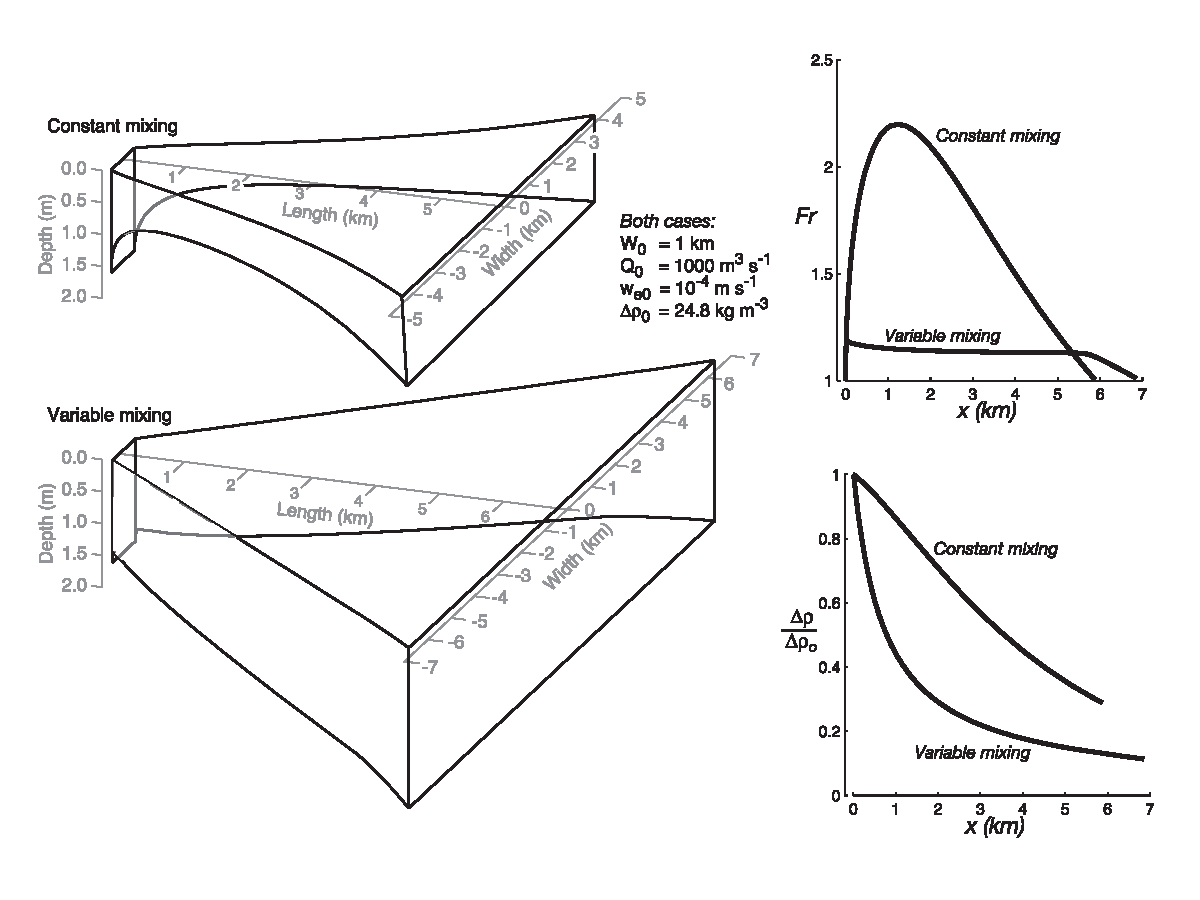
\includegraphics[width=6.5in]{Figures/plume3d_Fr_dr.pdf}
    \caption{Two idealized near-field plume simulations using constant entrainment, $w_e=w_{e0}$, and the Ellison and Turner (1959) parameterization, with a background (minimum) mixing of $w_{e0}$. The density anomaly and Froude number along the axis of each plume is shown to the right.}
    \label{fig:plume3d_Fr_dr}
\end{figure}

\subsection{Plume frontal mixing}

Near-field plume fronts can be regions of intense overturning and mixing. Observations of the Columbia River tidal plume show that fresh water at the plume front can plunge to 30 m below the free surface, about three times the thickness of the plume. Measurements in the Connecticut river plume also show the plume front being about twice that of the plume, though the plume is much thinner at about a meter \citep{odonnell.ea:98} While direct measurements of overturning and resultant mixing have so far not been possible due to the rapid translation of the plume front, analogies to gravity current bore heads suggest that mixing is intense.

Despite the fact that mixing at the front is clearly very intense, there is ongoing debate about what percentage of total net mixing within the plume that occurs at the plume front versus the supercritical flow region behind the plume front. \citet{pritchard.huntley:06} suggest that essentially all of the near-field plume mixing occurs within the front; \citet{orton.jay:05} suggest about 20\% of net mixing occurs within the Columbia plume front; \citet{cole:14} found even less net mixing within the plume front in a series of idealized experiments.

To further emphasize the ambiguity in the interaction between the quasi-steady plume and plume front, idealized experiments using steady fresh water forcing suggest that as the plume front propagates, it exposes a steady near-field plume in it's wake. Thus, studies of mixing within a plume have used both perspectives of flow through a steady plume \citep{hetland:10a}, or a Lagrangian perspective following the plume front \citep{jay:??}. Though conceptually distinct, there is considerable overlap in the analytical methods used to solve these two problems.

\subsection{Rotation and return to geostrophy}

High Froude numbers within a near-field plume imply strong advection. Thus high Froude numbers are generally associated with high Rossby numbers, $Ro = U (f L)^{-1}$, which in turn implies that rotation may not be a dominant factor in the flow. A key factor is the timescale of flow through the near-field; if this timescale is on the order of, or longer than, the rotational timescale $f^{-1}$, the flow will likely be influenced by rotation. In practice, the timescales of flow through a near-field plume are rarely greater than an hour, so the the impact of rotation is primarily to lean the plume toward the downcoast direction, as defined by the direction of coastal Kelvin wave propagation. But the result of even this minor influence of rotation is that spreading may be suppressed by the turning of the plume so that net plume mixing may be reduced as compared to a non-rotating plume \citep{cole.hetland:16}.


% \begin{itemize}
%   \item Plume structure and processes acting inside the plume
%   \begin{itemize}
%     \item 
%   \end{itemize}
%   \item Plume frontal processes
%   \item Relative importance
% \end{itemize}



% Observationss

% \cite{wright.coleman:71}
% \cite{kilcher.nash:10}
% \cite{jay.ea:10}
% \cite{stashchuk.vlasenko:09}
% \cite{nash.ea:09}
% \cite{pritchard.huntley:06}
% \cite{garvine:91,garvine:87,garvine:84,garvine:82,garvine:74b,garvine:74}
% \cite{jay.ea:inpress}
% \cite{hetland.macdonald:08}
% \cite{chen.macdonald:06,orton.jay:05,nash.moum:05}
% \cite{pritchard.huntley:02}
% \cite{odonnell:90}
% \cite{odonnell.ea:98}

% \section*{Acknowledgements}


\bibliographystyle{plainnat}
\bibliography{hetland}

\clearpage
\listoffigures

\clearpage
%%% FIGURES

\begin{figure}
    \centering
    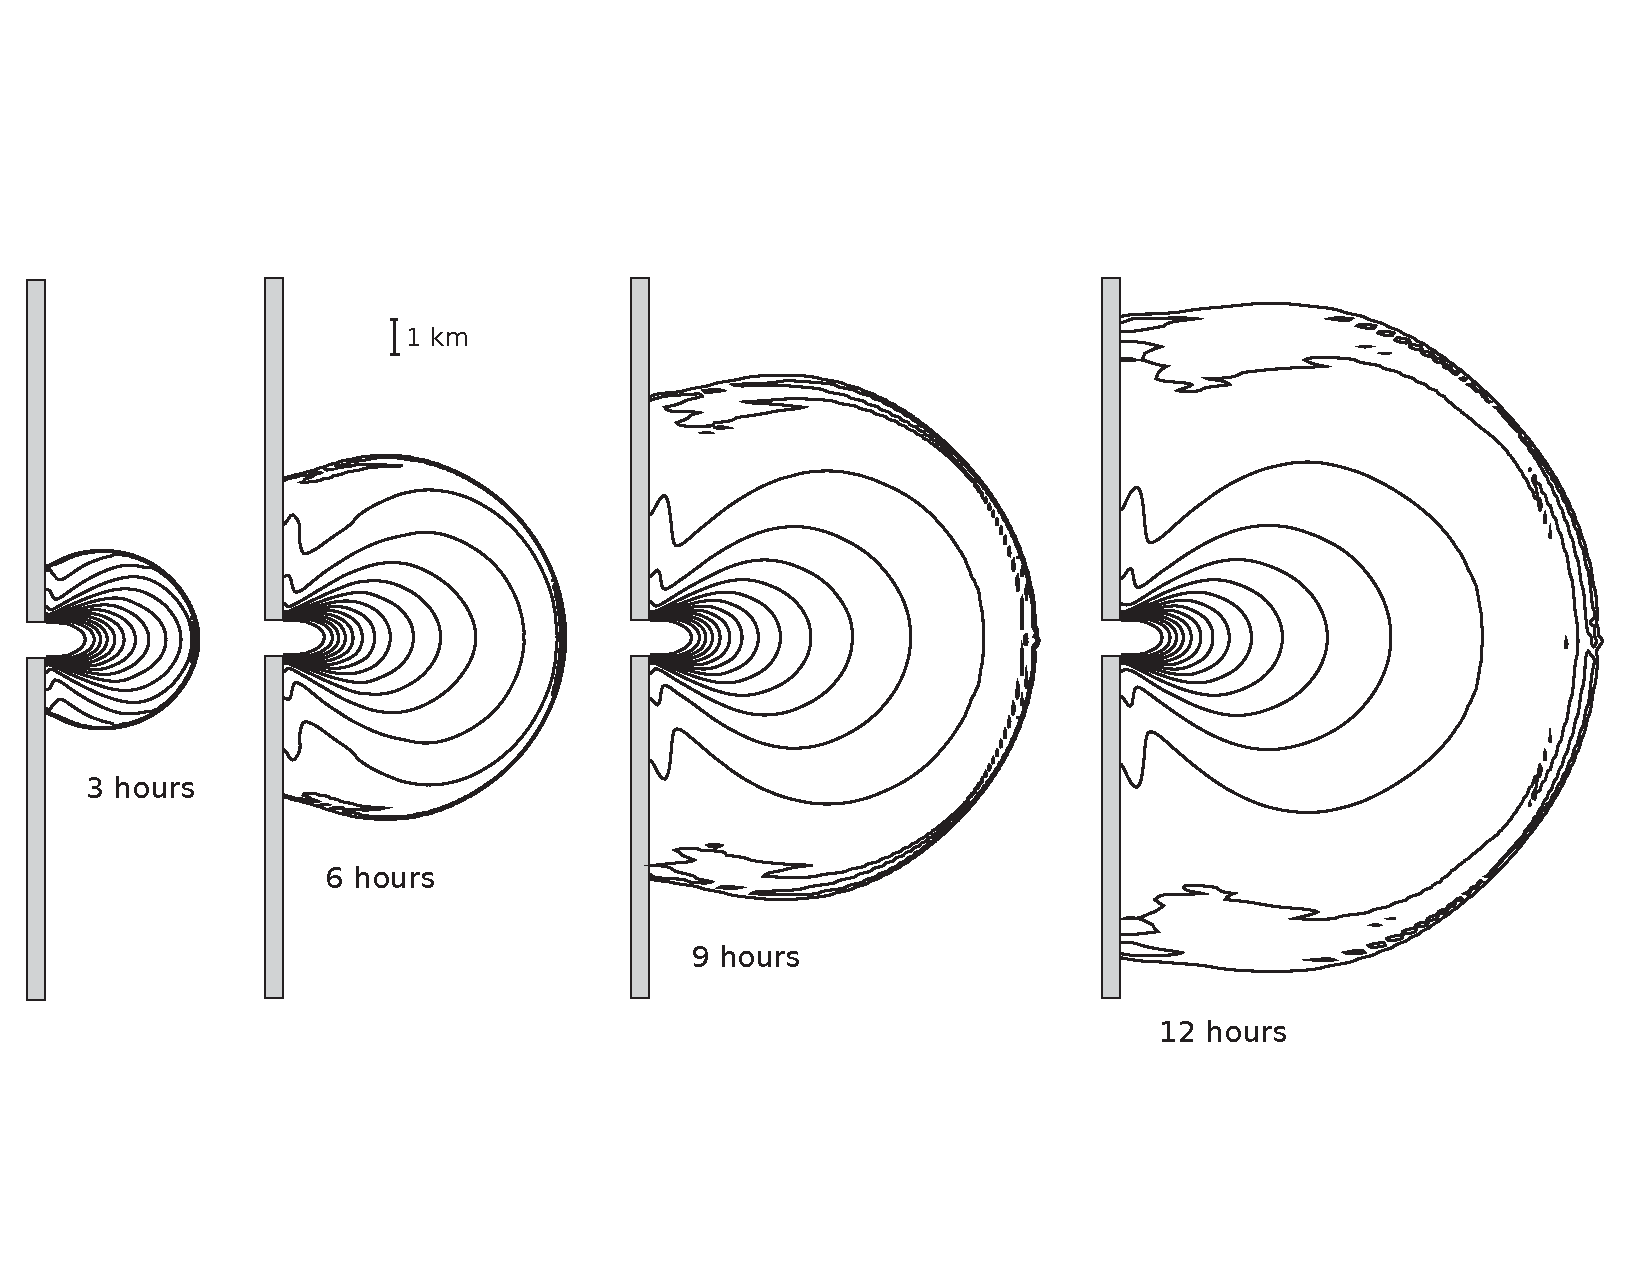
\includegraphics[width=6in]{Figures/plume_expansion_frames.pdf}
    \caption{Surface density contours are shown at four stages of plume evolution from a three-dimensional, non-linear hydrodynamic simulation using an idealized configuration.}
    \label{fig:3d_expansion}
\end{figure}

\begin{figure}
    \centering
    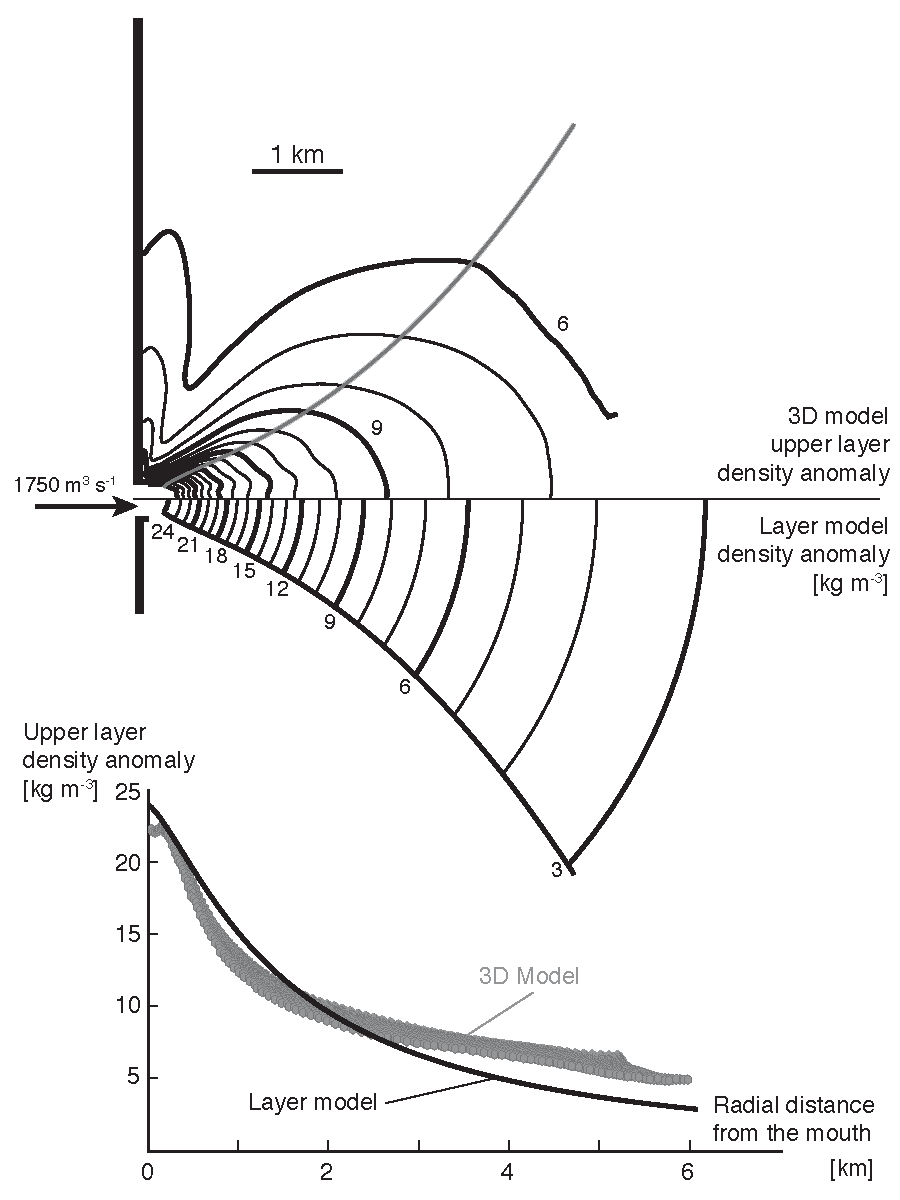
\includegraphics{Figures/ideal_comp_rev1.pdf}
    \caption{The top panel shows an example comparing a three-dimensional, non-linear hydrodynamic simulation (top half) with a corresponding idealized layer model (bottom half). The bottom panel shows the surface layer density from both models as a function of radial distance from the mouth at the time corresponding to the snapshot shwon in the upper panel.}
    \label{fig:my_label}
\end{figure}



\end{document}

